\graphicspath{{chapters/03/}}
\chapter{Analysis and interpretation of single cell sequencing data}

scRNA-sequencing is mainly applied for:

\begin{itemize}
\tightlist
\item
  \emph{discrete analysis}: identify new cell types and states within
  tissues and organs (in physiology and disease) → clustering
\item
  \emph{continuous analysis}: understand development paths (e.g.,
  embryonic development) and differentiation decisions (e.g.,
  hematopoiesis) → trajectory reconstruction
\end{itemize}

\begin{figure}
\centering
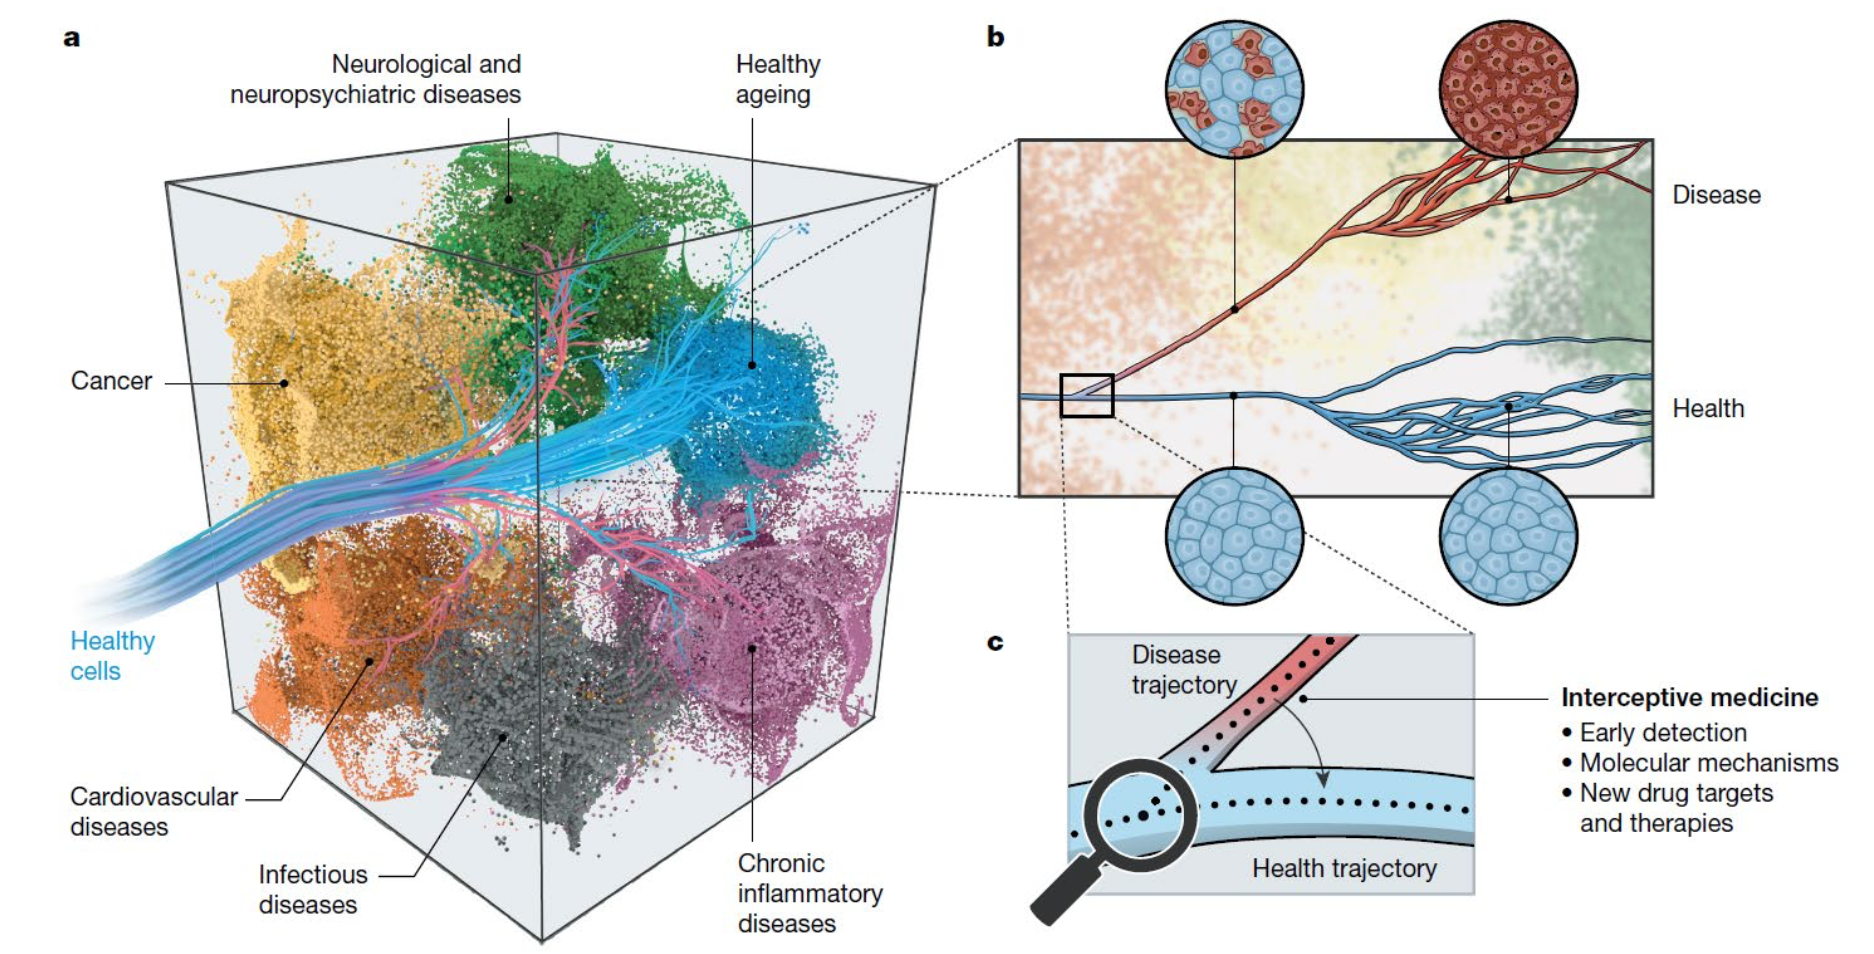
\includegraphics[width=0.5\textwidth]{images/Screenshot.png}
\caption{Rajewsky et al, Nature 2020}
\end{figure}

Example from perspective paper (\emph{Rajewsky et al, Nature 2020)}:
cells in our bodies are transitioning in age-related differentiation
trajectories. The idea is to investigate altered trajectories due to
disease e.g.~neurological, cancer, cardiological, infection
diseases\ldots{} in order to gain knowledge on the roots of disorders.
Ideally, we should identify the initial causes through early detection
and immediately intervene so as to prevent disease development.

\hypertarget{pre-processing}{%
\section{Pre-processing}\label{pre-processing}}

\hypertarget{from-raw-reads-to-count-matrices}{%
\subsection{From raw reads to count
matrices}\label{from-raw-reads-to-count-matrices}}

Reads are composed of:

\begin{itemize}
\tightlist
\item
  cDNA sequences (around 50 bp) corresponding to the original RNA
  fragments
\item
  technical region: cell barcode to understand the cell of origin
  (e.g.~10x sequence is 12 nt long) + UMI random sequence to remove
  possible technical artifacts e.g.~PCR duplicates
\end{itemize}

Through cDNA alignment and barcode ordering we can divide reads by cell
of origin and map them to a reference genome. By counting unique UMIs
for each gene in each cell we reach the \emph{count matrix}.

Raw sequencing data output depend on the sequencing platform, which is
usually Illumina, and are encoded in FASTQ format, which reports a title
(\texttt{@title}), sequence and a quality score for each base - PHRED
quality scores encoded as ASCII characters(ASCII 33-126). The title can
contain additional technical information as cell barcodes and UMI,
useful for downstream analysis. Unique molecular identifier reduce the
amplification noise by allowing (almost) complete de-duplication of
sequenced fragments. It is possible to trim a portion of the read or
discard the read itself according to quality PHRED scores.

The available alignment methods can be divided into two main categories:

\begin{itemize}
\tightlist
\item
  \textbf{splice-aware alignment tools:} map sequences derived from
  non-contiguous genomic regions, e.g.~spliced sequence modules (exons)
  that are joined together to form spliced RNAs e.g.~TopHat, HISAT2,
  STAR. STARsolo was developed for scRNA-seq, and is able to deal with
  cell barcodes and UMIs. The alignment output is saved as SAM/BAM file,
  which specifies where the read aligns and how the nucleotides in the
  read match up with the nucleotides in the target sequence (genome or
  transcriptome).
\item
  \textbf{pseudo-alignment tools:} the output file provides a set of
  target sequences that the read is compatible with. Advantage: provide
  accurate expression estimates very quickly and using little memory
  e.g.~Kallisto, SALMON. Example: kallisto \textbar{} bustools provides
  a workflow for association of reads with cell of origin, collapsing of
  reads according to UMIs and generation of a cell x gene matrix.
\end{itemize}

Many of the tools developed for bulk RNA-seq released versions suitable
for single cell specificity. Transcription factors are usually not
detected in single cell, so it is required to perform enrichment to
analyze them.

Reads could map to more than one location as the result of homolog genes
or transcribed transposable elements; an easy solution to this is to
increase read length.

An example of analysis pipeline is CellRanger (10X Genomics), which
processes Chromium single-cell data to align reads (with STAR), generate
count matrices, and other secondary analyses on Linux systems.

Differently from bulk count data, scRNA matrices report gene counts as
rows per cell (columns). The high presence of zeros could be due to true
lack of expression or technical lack of detection.

\begin{figure}
\centering
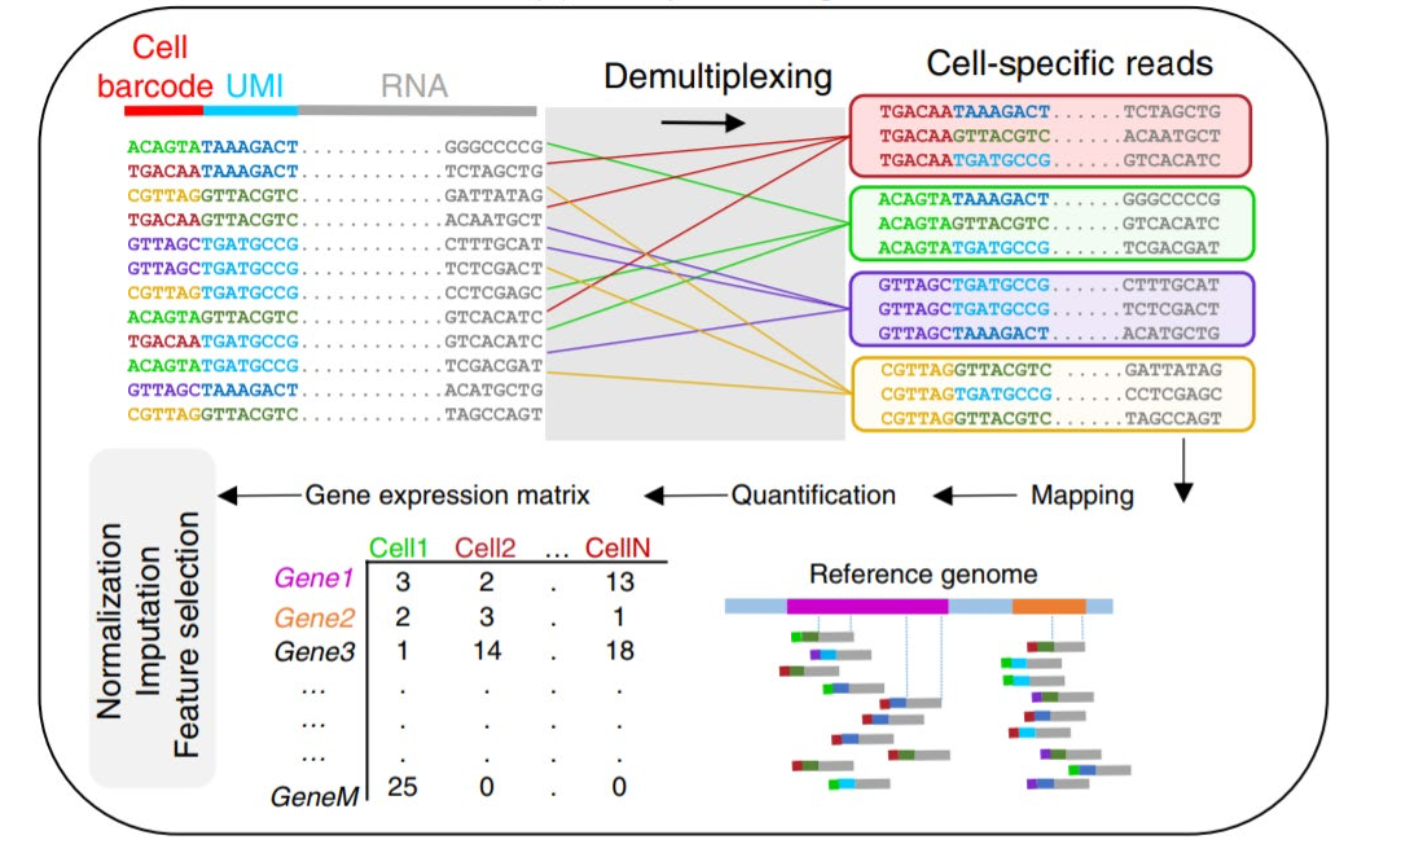
\includegraphics[width=0.5\textwidth]{images/Screenshot-1.png}
\caption{\emph{Lafzi A et al., Nature Protocols 2018}}
\end{figure}


\begin{figure}
\centering
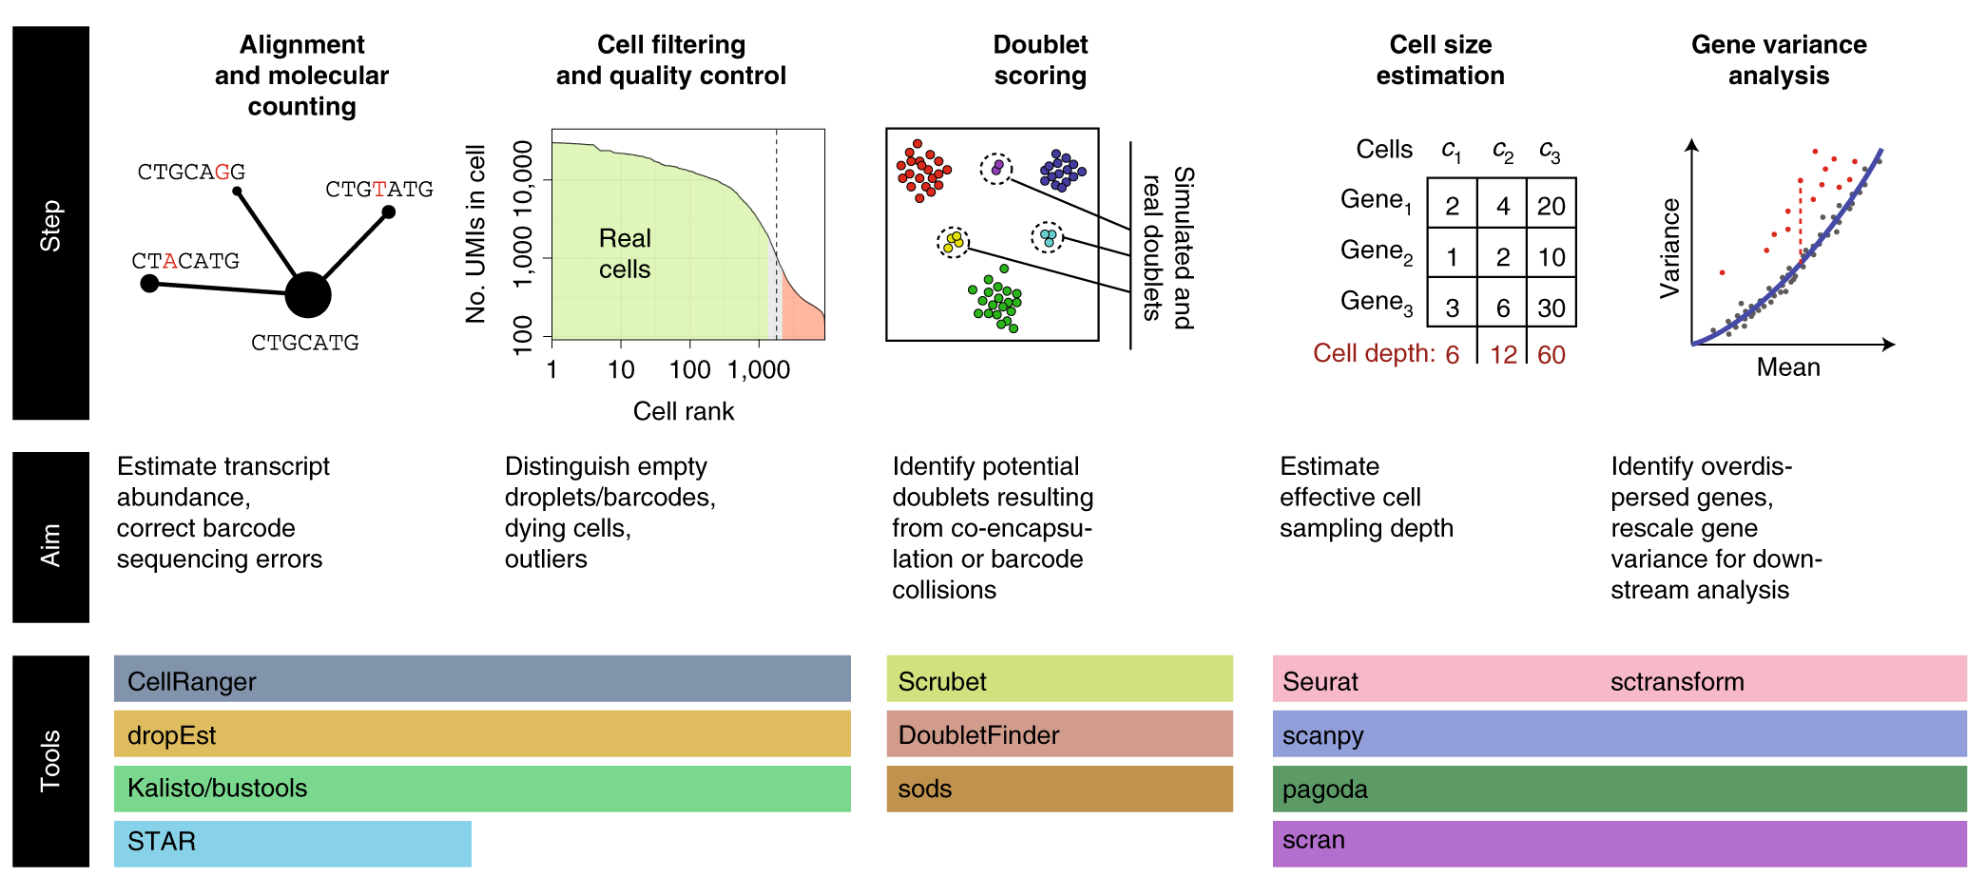
\includegraphics[width=0.5\textwidth]{images/Screenshot-2.png}
\caption{Kharchenko, P.V. \emph{Nat Methods} (2021).}
\end{figure}


\hypertarget{quality-control}{%
\subsection{Quality control}\label{quality-control}}

Cells with a low number of UMIs or reads can be filtered out (unless
linked to known biological features). The threshold can be based on a
quantile or on a distribution. Another check can be applied on the
number of mitochondrial genes; there are around \textasciitilde{} 40
mitochondrial genes and we should not see many mitochondrial genes in
single cell sequencing in general, as they are contained in mitochondria
and not in cytoplasm. Dying cells usually have high mitochondrial reads
due to the breakage of mitochondria and can hence be filtered out.

\begin{enumerate}
\def\labelenumi{\arabic{enumi}.}
\tightlist
\item
  remove low quality cells or empty droplets/dying cells. This is
  performed by isolating low UMIs (i.e.~low number of genes detected)
  and identifying extensive mitochondrial contamination (dying cells).
\item
  detect and remove doublets: experimental evaluation of doubles can be
  applied to measure the probability of doublets (2 or more cells
  included in a single droplet). In silico simulation e.g.~DoubletFinder
  (R) or Scrublet (Python) is performed as following:

  \begin{enumerate}
  \def\labelenumii{\arabic{enumii}.}
  \tightlist
  \item
    simulate thousands of doublets by adding together two randomly
    chosen profiles
  \item
    for each original cell, compute the density of simulated doublets in
    the surrounding neighborhood, and the density of other original
    cells in the neighborhood.
  \item
    return the ratio between the two densities as a ``doublet score''
    for each cell
  \end{enumerate}
\end{enumerate}

\hypertarget{normalization}{%
\subsection{Normalization}\label{normalization}}

The aim is to remove systematic/technical differences in sequencing
coverage between cells. The simplest approach to achieve this is library
size normalization, where we divide for the total sum of counts across
all genes for each cell. This method is based on the questionable
assumption that each cell should have the same number of reads; we could
have issues with highly expressed genes. In addition, this method does
not normalize well highly expressed genes; by binning genes in different
classes according to average expression, it was seen that the higher the
n of reads, the higher the number of of genes also after correction.
Hence, the same normalization approach for each gene is not the same
solution. We could improve by following one of these approaches:

\begin{enumerate}
\def\labelenumi{\arabic{enumi}.}
\tightlist
\item
  \textbf{uniform scaling per cell}: identify ``size factors'' for
  individual cells, applied to all genes

  \begin{itemize}
  \tightlist
  \item
    sing bulk RNA-seq methods (TMM in edgeR, DESeq2) (problem with
    excess of 0s)
  \item
    using spike-ins RNAs (e.g., ERCC) (assumption: same amount of
    spike-in in each cell) (BASiCS, Vallejos et al, PLOS Comp Biol 2014)
  \item
    pooling cells with similar library sizes and estimate pool-based
    size factors (scran, Lun et al, Genome Biology 2016)
  \end{itemize}
\item
  \textbf{Gene or gene-group scaling factors}: different scaling factors
  for groups of genes with high, medium and low abundance

  \begin{itemize}
  \tightlist
  \item
    SCnorm (Bacher et al, Nature Methods 2017)
  \item
    Sctransform (Hafemeister et al, Genome Biology 2019)
  \end{itemize}
\end{enumerate}

Keep in mind that normalization choices likely affect results! As an
example, we can analyze the t-SNE plots of mouse lung epithelial cells
(3 embryo stages + adult cells) under various normalization methods.
Simple Norm is the library size normalization, BASiCS, GRM, SAMstrt
require spike-in RNAs and Linnorm, Scnorm, scran do not require spike-in
RNAs.

\begin{figure}
\centering
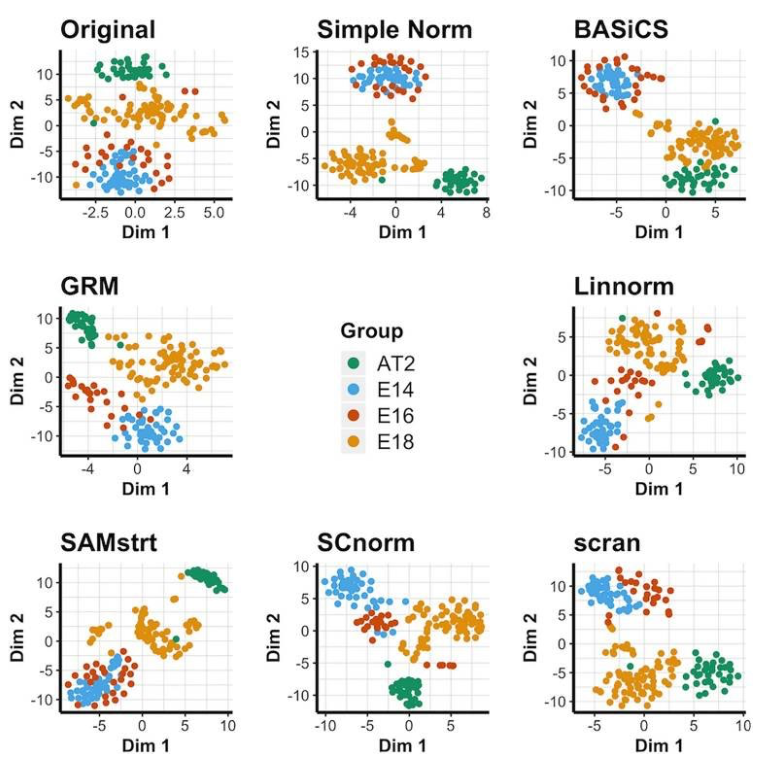
\includegraphics[width=0.5\textwidth]{images/Screen_Shot_2023-02-22_at_15-08-31.png}
\caption{\emph{Lytal N, Ran D, An L. Normalization Methods on
Single-Cell RNA-seq Data: An Empirical Survey. Front Genet. 2020}}
\end{figure}

Good practice entails applying different methods and choose a consensus,
as normalization deeply impacts downstream analysis.

\hypertarget{analysis}{%
\section{Analysis}\label{analysis}}

\begin{figure}
\centering
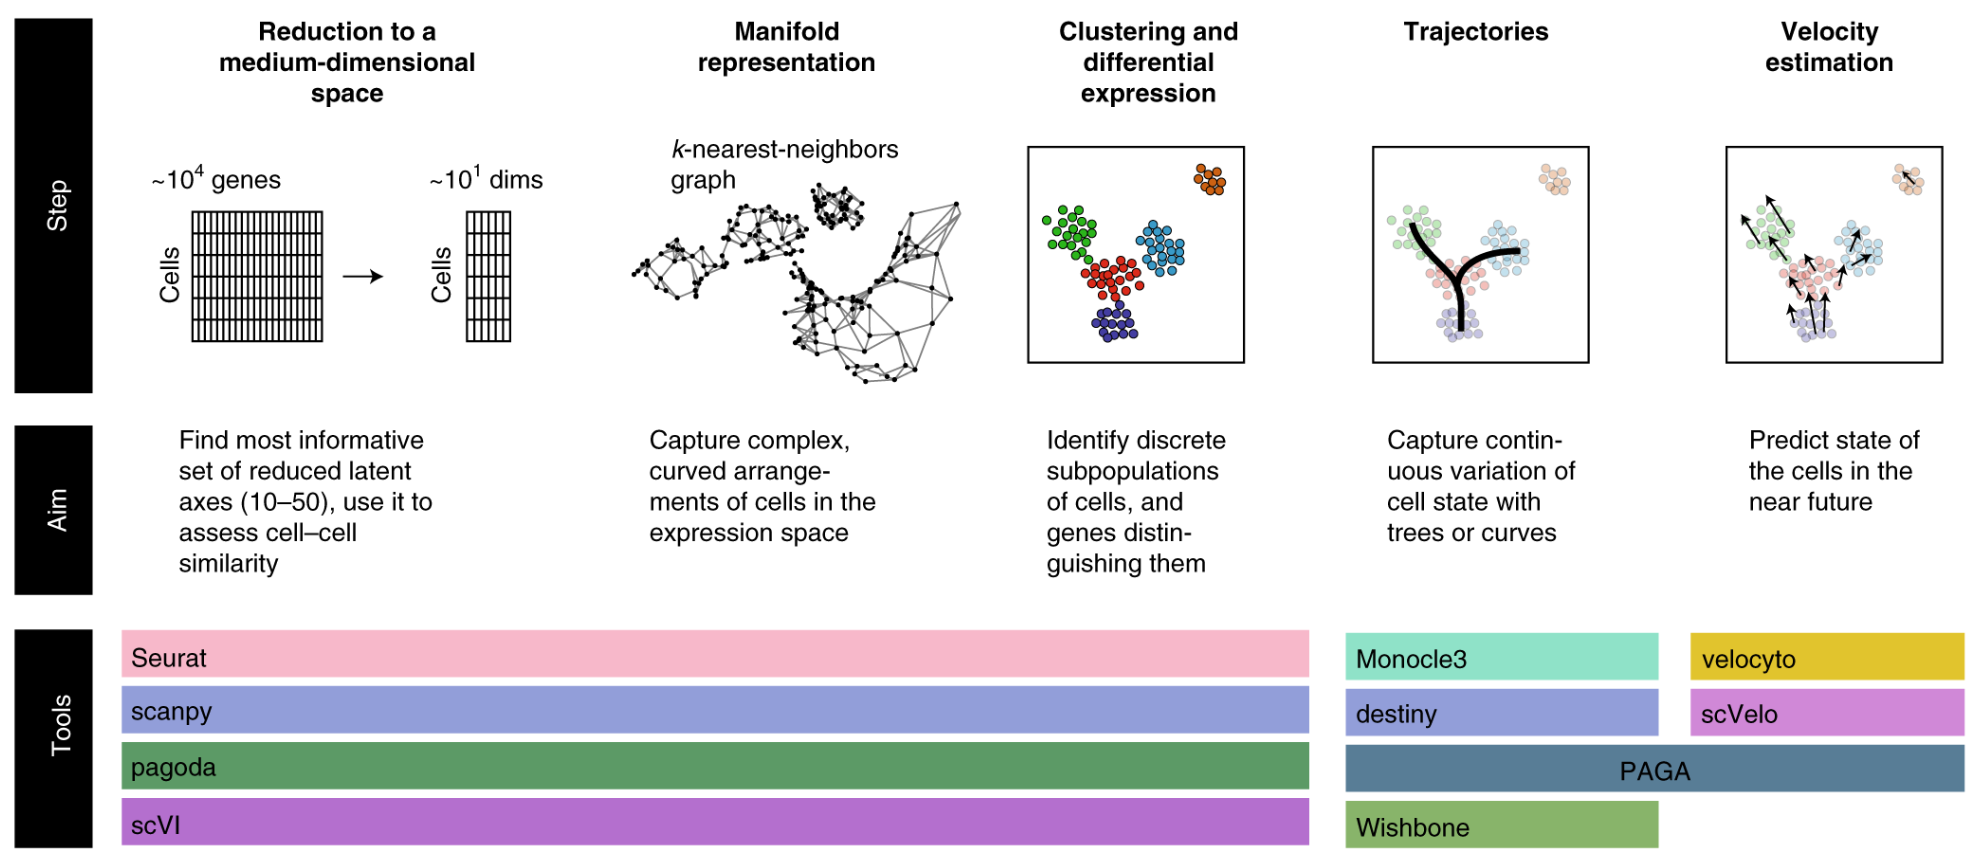
\includegraphics[width=0.8\textwidth]{images/Screenshot-3.png}
\caption{Kharchenko, P.V. \emph{Nat Methods} (2021)}
\end{figure}

\hypertarget{dimensionality-reduction}{%
\subsection{Dimensionality reduction}\label{dimensionality-reduction}}

Problem: a typical scRNA-seq data table consists of
\textasciitilde20,000 genes as features and 10,000 to up to a million
cells as observations. We can reduce the number of features to reduce
data complexity and ease the visualization of cells. This approach is
based on the notion that not all genes are important to classify cells
(\emph{gene/feature selection}) and several genes are correlated in
expression (\emph{redundancy}).

Gene (feature) selection:

\begin{itemize}
\tightlist
\item
  select genes that contain useful information about the biology of the
  system
\item
  remove genes that contain random noise or do not vary among cells
\item
  reduce the size of the data, improve computational efficiency
\end{itemize}

The simplest approach is to select the most variable genes based on
their expression across the population of cells. However, the underlying
assumption is that biological variability is higher than technical.

Dimensionality reduction:

\begin{itemize}
\tightlist
\item
  reduce the number of separate dimensions in the data
\item
  help downstream analyses (clustering, trajectory inference \ldots)
\item
  help the visualization of data in 2D plots
\end{itemize}

Multiple methodologies are available, with different advantages and
limitations. In Principal Component Analysis the expression of each gene
is a dimension and the goal is to center data and express the variation
associated with each dimension, such that cells are represented on the
line that captures more variation.

\begin{itemize}
\tightlist
\item
  PCA: Principal Component Analysis (linear)

  \begin{itemize}
  \tightlist
  \item
    pros: highly interpretable and computationally efficient
  \item
    cons: inappropriate for scRNA-seq visualization (non-linear data,
    excess of 0s).
  \end{itemize}
\end{itemize}

PCA is not the optimal way to visualize single cell data, as groups tend
to be more mixed and the overall result is less interpretable, due to
the high presence of zeroes in the matrix. To solve the issue, two main
methods were developed for dimensionality reduction visualization:

\begin{itemize}
\tightlist
\item
  \textbf{t-SNE}: t-Stochastic Neighbourhood Embedding (non-linear,
  graph-based)

  \begin{itemize}
  \tightlist
  \item
    pros: able to retain the local structures in low dimensions
  \item
    cons: stochastic method, long time to run with high n, global
    structure of data is not preserved
  \end{itemize}
\end{itemize}

The main issue of t-SNE is that it does not scale well with data (works
best with 2 or 3 dimensions which should be established beforehand) and
cannot maintain well the structure of the dataset (randomness).

\begin{itemize}
\tightlist
\item
  \textbf{UMAP}: Uniform Manifold Approximation and Projection
  (non-linear, graph- based)

  \begin{itemize}
  \tightlist
  \item
    pros: computationally efficient, better preservation of global
    structure
  \item
    cons: low interpretability, stochastic method
  \end{itemize}
\end{itemize}

From 2018, the gold standard is UMAP, as it manages to preserve the
global structure and is computationally efficient (compromise among PCA
and t-SNE). Each run could still give different results due to
stochasticity, but due to the fact that the initial steps are non-random
there is more stability with respect to t-SNE.

\begin{figure}
\centering
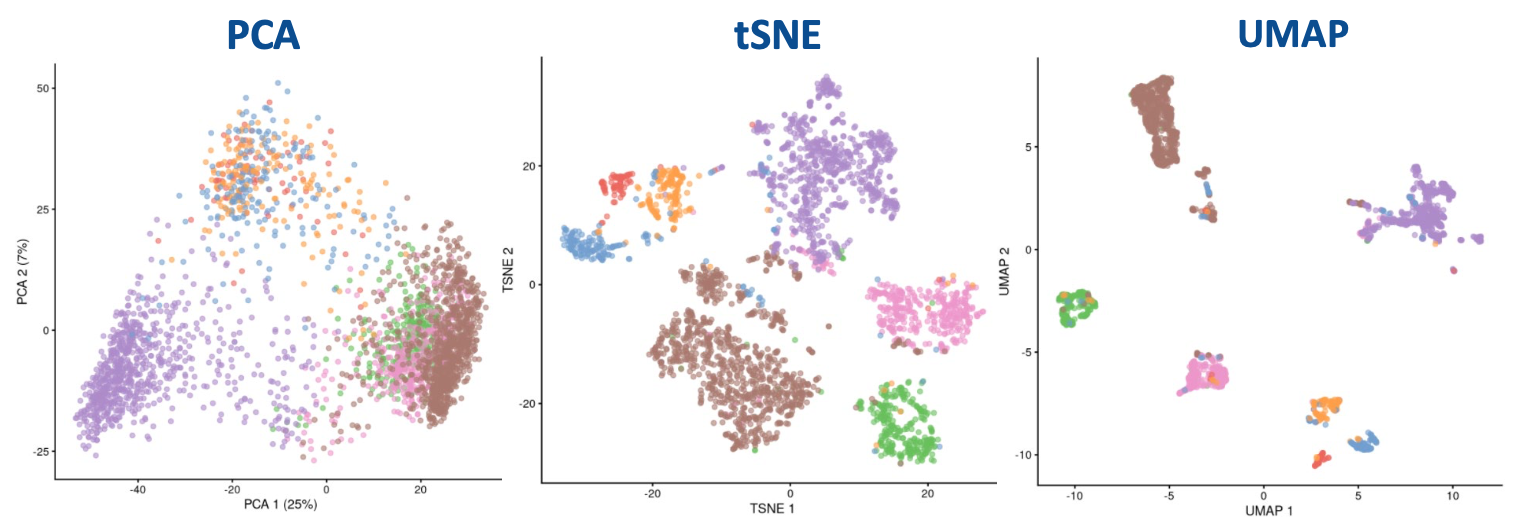
\includegraphics[width=0.5\textwidth]{images/Screen_Shot_2023-02-22_at_15-18-21.png}
\caption{Screen Shot 2023-02-22 at 15-18-21.png}
\end{figure}

\hypertarget{clustering}{%
\subsection{Clustering}\label{clustering}}

For characterizing cell states it is required to organize cells
according to their identity, which could be shaped by environmental
stimuli, cell development, cell cycle or spatial context. Through single
cell, it is possible to detect such changes through discrete analysis or
continuous approaches (developmental trajectory or circle path).

Clustering approaches developed for data sciences can be applied to
single cell data e.g.~hierarchical clustering, K-means or graph-based
approaches (most used as they are particularly suited for high
dimensional data). The aim is to identify highly interconnected
communities within the population. Algorithms identify the edges that,
when remove, result in a higher difference among groups. It is possible
to weight edges according to cell similarity e.g.~Euclidean distance or
according to their neighbourhood e.g.~if they share neighbouring points.

In \textbf{graph-based approaches}, each node is a cell connected to its
nearest neighbors in the high-dimensional space. Edges are weighted
based on the similarity between the 2 cells. The strategy focuses on
identify ``communities'' of cells that are more connected to cells in
the same community than they are to cells of different communities. A
popular approach is the Louvain method for community detection.

Once clusters are identified, the aim is to characterize clusters
according to differential expression. Issue: heterogeneity in gene
expression distribution makes it hard to use parametric methods →
non-parametric choices are a solution. In order to identify genes with
different expression among clusters of cells, hence to distinguish
cluster markers, we can apply:

\begin{itemize}
\tightlist
\item
  non-parametric tests (Wilcoxon Rank Sum test) → problematic with tied
  values (0s)
\item
  methods inherited from bulk RNA-seq (edgeR, DESeq2, based on negative
  binomial models)
\end{itemize}

Transform negative binomial to zero inflated negative binomial to
account for the high presence of zeroes in the matrix. {[}!added
slide{]}

\begin{itemize}
\tightlist
\item
  methods developed for single cell (dealing with the excess of 0s)
\end{itemize}

In Seurat package we have the \ldots{} function with default Wilcoxon,
but it is possible to use other methods e.g.~ROC curve with marker
genes.

\hypertarget{t-test-differential-expression}{%
\subsubsection{t-test differential
expression}\label{t-test-differential-expression}}

With the t-test, we must apply the assumption of Normal distribution
i.e.~we should see a low variability in differentially expressed genes.
The null hypothesis states that the mean of the control and the
treatment is equal, in other words, the distribution of the mean should
be normal. We compute the t-test as:

\[
t=\frac{\bar{X_T}-\bar{X_C}}{\sqrt{\frac{\text{var}_T}{\text{n}_T}+\frac{\text{var}_C}{\text{n}_C}}} \\ \frac{\text{signal}}{\text{noise}} = \frac{\text{difference between group means}}{\text{variability  of groups}}
\]

The p-value is the probability for a given statistical model that, when
the null hypothesis is true, the statistical summary (e.g.~t-statistic)
would be the same as or more extreme than the actual observed results.
It can be seen graphically as the sum of tail areas in the two-tailed
test.

\hypertarget{non-parametric-tests}{%
\subsubsection{Non-parametric
tests}\label{non-parametric-tests}}

In non-parametric tests, expression values are ranked from lowest to
highest without making assumptions on the distribution of the data. The
sum of the ranks for each group is used to check the difference among
clusters, which is associated with a pvalue; if the rank sums are very
close, the pvalue will not be significant.

\textbf{Wilcoxon Rank-Sum} test aka \textbf{Mann-Whitney U test} convert
observed expression values to ranks, and test whether the distribution
of ranks for one group are significantly different from the distribution
of ranks for the other group. In this case there is no assumption on the
distribution of data, but it could be problematic with tied values (0s).

\hypertarget{multiple-test-correction-methods}{%
\subsubsection{Multiple test correction
methods}\label{multiple-test-correction-methods}}

High-throughput results usually have multiple comparison problem, due to
expression variation (thousands of genes) and pathway enrichment
(hundreds of pathways). The obtained raw pvalues can be corrected to
minimize false positives. For instance, with a pvalue threshold of 0.05
in a setting of 10k genes, we expect that 500 genes are false positive,
generating a very high false discovery rate. For reducing FP in
selection, it is possible to apply multiple test correction methods. For
instance, with Bonferroni correction we can increase the original
p-values to reduce false positives - do not swap the order of the
original p-values.

\begin{itemize}
\item
  \textbf{Bonferroni correction}: multiply the original p-value for the
  number of tests performed (M). It controls the probability to have at
  least 1 false positive result (controlling the Family Wise Error Rate
  FWER). It is a very stringent and conservative correction, especially
  with large numbers of tests → possibly leads to false negatives.

  \(\text{adjusted P value} = (\text{original P value}) \times (\text{number of tests})\)
\item
  \textbf{Benjamini Hochberg correction}: most popular multiple test
  correction method, introduced in 1995. It was designed to control the
  False Discovery Rate (FDR), the expected proportion of ``false
  positives''. It is a stepwise method, as it requires to sort all
  original p-values in increasing order and determine the rank (1,2,3,
  \ldots)

  \(\text{adjusted P value} = (\text{original P value}) \times (\frac{\text{number of tests}}{\text{P value rank}})\)
\end{itemize}

\hypertarget{cell-type-annotation}{%
\subsection{Cell type annotation}\label{cell-type-annotation}}

For annotating clusters with known cell types we can proceed with:

\begin{itemize}
\tightlist
\item
  manual approach, based on personal knowledge
\item
  automatic approach, based on:

  \begin{itemize}
  \tightlist
  \item
    databases of marker genes e.g.~Panglaodb or CellMarker
  \item
    cell type expression data e.g.~bulk RNA-seq
  \item
    labeled scRNA-seq datasets
  \end{itemize}
\end{itemize}

\hypertarget{annotation-based-on-marker-genes-sctype}{%
\subsubsection{\texorpdfstring{\textbf{Annotation based on marker genes
(scType)}}{Annotation based on marker genes (scType)}}\label{annotation-based-on-marker-genes-sctype}}

Score based on the scaled expression of marker genes (z-scores)

\begin{enumerate}
\def\labelenumi{\arabic{enumi}.}
\tightlist
\item
  Calculation of marker specificity scores (weights)
\item
  Use of positive\&negative markers
\end{enumerate}

\hypertarget{reference-based-annotation-singler}{%
\subsubsection{Reference based annotation
(SingleR)}\label{reference-based-annotation-singler}}

SingleR is a protocol for cell type annotation by reference to
transcriptomes of pure cell types(score based on Spearman correlation)

\hypertarget{integration-of-single-cell-datasets}{%
\subsection{Integration of single cell
datasets}\label{integration-of-single-cell-datasets}}

The goal is to remove batch effects and confounders. Through the Seurat
package we can perform \textbf{Canonical Correlation Analysis} (CCA),
which is able to capture correlated sources of variation between two
datasets.

If we are trying to classify cells according to gene expression, it is
required to use strictly gene expression markers. We do not want data to
be clustered according to platform or batch; we can apply different
integration approaches to solve the issue.

\textbf{Anchor based approaches}: reference and query dataset should be
integrated. We identify among the two datasets that are assumed to be in
the same state (similar to each other in a reduced space), which are
then used as anchors. The other cells will be corrected according to a
measure expressing how different the cells are from anchors and from the
dataset they belong to. This method works well while integrating similar
system, as most cells are assumed to align.

\begin{figure}
\centering
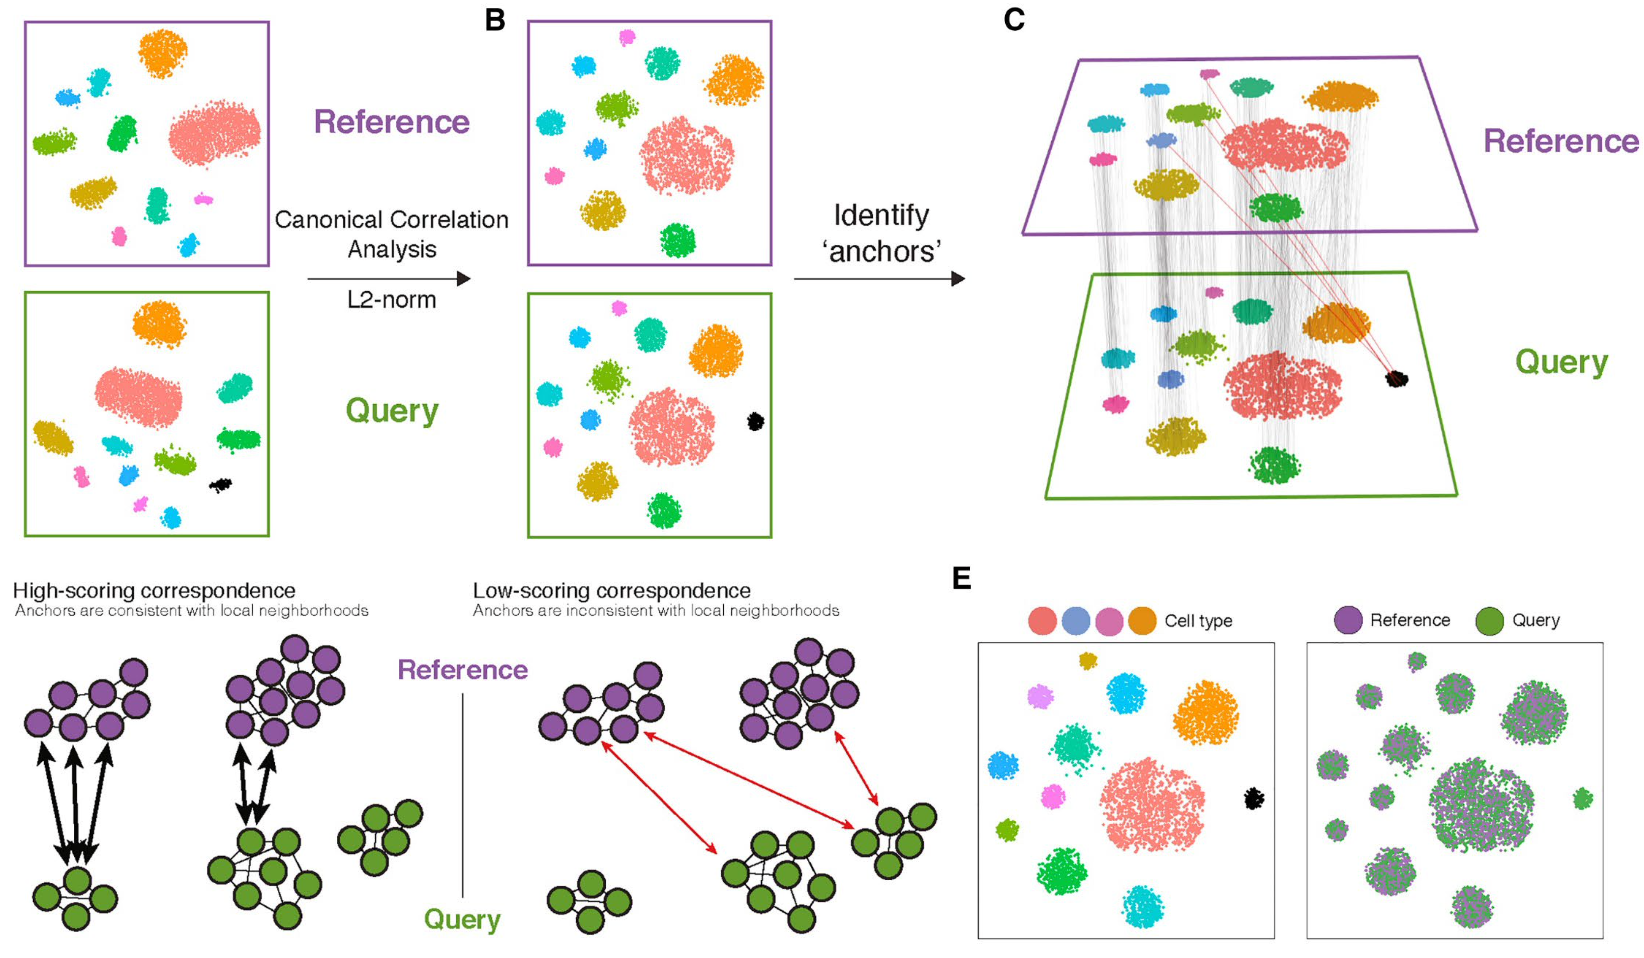
\includegraphics[width=0.5\textwidth]{images/Screenshot-4.png}
\caption{\emph{Stuart et al, Comprehensive Integration of Single-Cell
Data, Cell 2019}}
\end{figure}

Canonical Correlation Analysis is a linear method for dimensionality
reduction which can be compared to PCA, as it is also a linear
combination. Differently from PCA, the components will maximize the
correlation between two dataset. We can visualize the output of the two
methods on the same dataset in Figure \ldots{}

\hypertarget{trajectory-analysis}{%
\section{Trajectory analysis}\label{trajectory-analysis}}

Instead of dividing cells into discrete clusters, we can place cells
along a continuous path representing the evolution of a process
(e.g.~differentiation). The main assumption entails capturing all the
snapshots of the process as a continuous spectrum of states (with
intermediates). The meaningfulness of the reconstructed trajectory must
be evaluated carefully, as this method will always lead to a result
i.e.~any dataset can be forced into a trajectory.

One common approach is to build a minimum spanning tree over cells,
minimizing the total sum of the branches, or over cell clusters while
working with a high number of cells. In most methods, the choice of the
root is performed manually (usually based on markers and known
biological information). Next, each cell's \emph{pseudotime} is
calculated as its distance along the tree to the root.

\begin{figure}
\centering
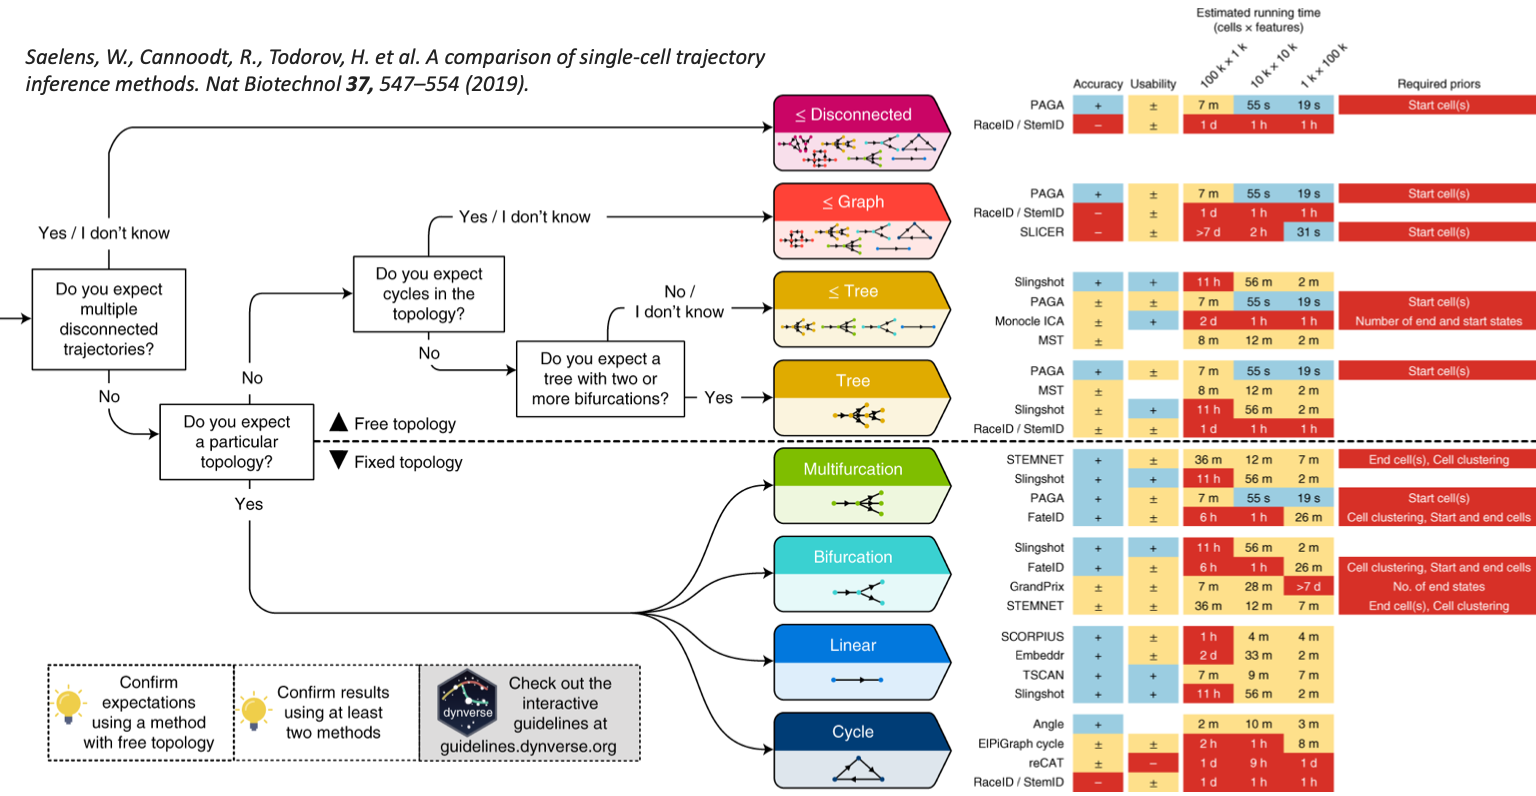
\includegraphics[width=0.5\textwidth]{images/Screen_Shot_2023-02-22_at_19-10-01.png}
\caption{}
\end{figure}

\hypertarget{monocle-2014}{%
\subsubsection{Monocle (2014)}\label{monocle-2014}}

Monocle R package provides tools for analyzing single-cell expression
experiments. In 2014, Cole Trapnell introduced the strategy of ordering
single cells in pseudotime, placing them along a trajectory
corresponding to a biological process such as cell differentiation.

Dataset of differentiation myoblasts (SMART-seq) in pseudotime. The
trajectory captures the transition from proliferating cells to
differentiated cells through interstitial mesenchymal cells. The method
has a high computational cost, so cannot be applied to huge datasets.

\hypertarget{monocle-2-2017}{%
\subsubsection{Monocle 2 (2017)}\label{monocle-2-2017}}

Monocle 2 is a method for finding trajectories through \textbf{reversed
graph embedding}. Each cell is represented as a point in high
dimensional space (x), where each dimension corresponds to the
expression level of an ordering gene. Data are projected onto a
lower-dimensional space by dimension-reduction methods such as PCA.

Monocle 2 constructs a spanning tree on a set of \emph{centroids}
(diamonds) chosen automatically using k-means clustering. Cells are
shifted toward the nearest tree vertex, vertex positions are updated to
`fit' cells, a new spanning tree is learned, and the process is iterated
until the tree and cells converge. The user then selects a tip as the
`root', and each cell's pseudotime is calculated as its \emph{geodesic
distance} along the tree to the root.

\begin{figure}
\centering
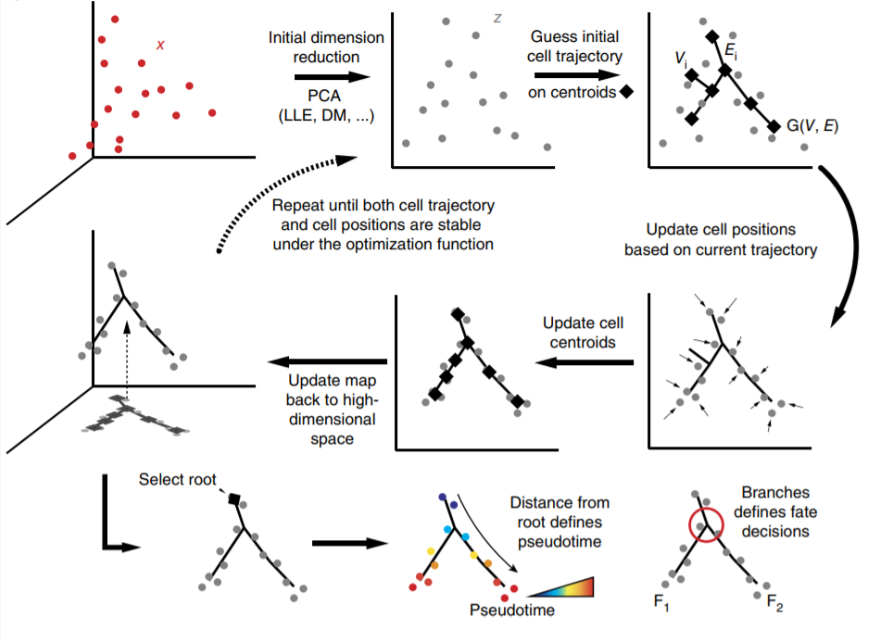
\includegraphics[width=0.5\textwidth]{images/Screen_Shot_2023-02-22_at_19-13-32.png}
\caption{\emph{Qiu X et al., Nature Methods 2017}}
\end{figure}


\hypertarget{comparing-dimensionality-reduction-and-ta-choices}{%
\subsubsection{Comparing dimensionality reduction and TA
choices}\label{comparing-dimensionality-reduction-and-ta-choices}}

Datasets with increasing number of cells are analyzed with different
approaches e.g.~PCA, UMAP, Monocle2,\ldots{} We can identify which
methods scale well with increasing numbers of cells.

\hypertarget{velocyto-2018}{%
\subsubsection{Velocyto (2018)}\label{velocyto-2018}}

\textbf{RNA velocity:} the time derivative of the gene expression state
(\(\frac{ds}{dt}=u- \gamma s\)) - based on the proportion of unspliced
vs spliced reads in single-cell RNAseq - predicts the future state of
individual cells on a timescale of hours. In other words, the balance
between unspliced and spliced mRNAs is predictive of cellular state
progression, where:

\begin{itemize}
\tightlist
\item
  \(u > \gamma s\) induction
\item
  \(u = \gamma s\) steady state
\item
  \(u < \gamma s\) repression
\end{itemize}

A read partially mapping an intron and exon is assumed to be
\emph{unspliced}. The whole method is based on the concept that the
ratio of spliced and unspliced reads can aid us in making hypotheses on
the future development of the cell. If the amount of unspliced reads is
higher than spliced we expect that we will reach a higher expression
level in the cell → transcription induction. Viceversa, a higher amount
of spliced reads characterizes repression of transcription.

RNA velocity is the time derivative of gene expression state based on
the proportion of unspliced vs spliced reads in scRNA-seq.

\textbf{Limitation}: same constants for all genes, incorrect assumption.
In addition, timescale could greatly vary in different processes
e.g.~hematopoiesis is not recapitulated well.

→ scVelo

! bias with 3'end approaches, not many introns → bias on splicing events
capturing

\hypertarget{scvelo-2020}{%
\subsubsection{scVelo (2020)}\label{scvelo-2020}}

The aim is to infer gene-specific rates of transcription, splicing and
degradation. scVelo provides a dynamical model, as it generalizes RNA
velocity to systems with transient cell states, common in development
and in response to perturbations.

\hypertarget{main-pitfallschallenges-in-current-scrna-seq}{%
\section{Main pitfalls/challenges in current
scRNA-Seq}\label{main-pitfallschallenges-in-current-scrna-seq}}

\begin{itemize}
\tightlist
\item
  Incomplete detection (`drop- out') of lowly expressed genes. Drop- out
  can blur fine-scale distinctions. Tentative solution: imputation
  methods.
\item
  Amplification bias (tentative solution: use of UMI)
\item
  Stochastic gene expression
\item
  Background noise
\item
  Bias due to cell size (smaller cells are more efficiently incorporated
  in droplets than large cells) and other factors (cell cycle)
\item
  Analysis restricted to polyA transcripts, no method for total RNA
  sequencing in single cells (solutions will be available soon)
\item
  dealing with high dimensionality

  \begin{itemize}
  \tightlist
  \item
    the number of cells included in average scRNA-seq is growing more
    than Moore's law. In the plot we can analyze the number of CPUs in
    the evolution of processors. The angular coefficient of the growth
    is higher than the increase in computational availability of
    processors → issue
  \end{itemize}
\item
  absence of standard methodologies
\item
  high variability of results, depending on methodologies and parameters
\end{itemize}

A lot of methods are based on graph-approaches. Example: changing
resolution deeply affects the results e.g.~granularity of clustering.
